\subsection{Un árbol de decisión simple}\label{simple}

Como punto de partida para nuestro análisis, vamos a entrenar un \textit{árbol de decisión} simple sobre los datos de entrenamiento. De esta manera, tendremos un piso respecto a la performance que podemos esperar de cualquier modelo a entrenar. Con \textit{simple} nos referimos a un modelo de poca complejidad, que sea fácilmente interpretable y propenso al \textit{underfitting} por contar con un sesgo inductivo alto\footnote{En otras palabras, cuyo espacio de hipótesis sea sencillo.}. De manera concreta, el árbol a entrenar tendrá una profundidad máxima de $3$ niveles y usará los hiperparámetros por defecto de la biblioteca \textit{scikit-learn}\footnote{Luego, las hipótesis representables tendrán la forma de conjunciones de a lo sumo tres comparaciones, donde cada comparación evalua algún umbral para algún atributo particular de las instancias.} para el \textit{DecisionTreeClassifier}.

Para estimar la performance del modelo utilizaremos $5$-fold cross validation estratificado\footnote{Ver la función \textit{cross\_val} en el notebook adjunto. Usamos el splitter \textit{StratifiedKFold} de \textit{scikit-learn}, con \textit{random\_state} $= s$. Para procurar que la comparación entre métricas sea justa, se reseteó el \textit{random\_state} entre corridas.} sobre $D_{train}$, para las métricas de \textit{accuracy}, \textit{aucroc} y \textit{auprc}. Mediremos la performance en entrenamiento y validación por split. También, tomaremos el promedio $\bar\phi$ en ambos casos y, para validación, realizaremos el cálculo del score global\footnote{Notar que todo $D_{train}$ fue parte del set de validación para alguna iteración de cross-validation. Luego, podemos calcular $$\Phi = metrica(\bigcup_{i=1}^5\text{Predict}(M^{(i)}, X_{cv_{validation}}^{(i)}), y_{train})$$ para estimar la performance del modelo sin recurrir a promedios.} $\Phi$.

% \vspace{0.5em}
% \begin{enumerate}
%     \item Dividimos el set de entrenamiento en $5$ grupos al azar, procurando que cada grupo mantenga la distribución de clases del set original\footnote{Usamos el splitter \textit{StratifiedKFold} de \textit{scikit-learn} con $k=5$ y \textit{random\_state} $= s$. Para procurar que la comparación entre métricas sea justa, se reseteó el \textit{random\_state} entre corridas.}: $$D_{train} \rightarrow (D_{train}^{(1)}, D_{train}^{(2)}, D_{train}^{(3)}, D_{train}^{(4)}, D_{train}^{(5)})$$
% 
%     \item Por turnos, consideramos un subconjunto como un set de \textit{validación} y al resto como un set de \textit{entrenamiento}.$$
%     cv^{(i)} = (D_{cv_{train}}^{(i)},\ D_{cv_{validation}}^{(i)}) = (D_{train}^{(i)},\ \bigcup_{j \neq i} D_{train}^{(j)})\ \ \forall i: 1 \dots 5$$
% 
%     \item Por cada par $cv^{(i)} $, entrenamos un \textit{árbol de decisión} simple, con los hiperparámetros descriptos: $$M^{(i)} = \text{Train}(Arbol,\ D_{cv_{train}}^{(i)})$$
%     
%     \item Evaluamos la performance de cada modelo $M^{(i)}$ sobre $cv^{(i)}$, utilizando la métrica seleccionada: 
%     \begin{align*}
%         \phi_{train}^{(i)} &= \text{metric}(\text{Predict}(M^{(i)}, X_{cv_{train}}^{(i)}), y_{cv_{train}}^{(i)})\\
%         \phi_{validation}^{(i)} &= \text{metric}(\text{Predict}(M^{(i)}, X_{cv_{validation}}^{(i)}), y_{cv_{validation}}^{(i)})
%     \end{align*}
%     \item Tomamos el promedio de las evaluaciones, para tener un primer estimado del desempeño del modelo, independiente de $D_{train}$. Es decir, un estimación \textit{realista} de la performance:
%     \begin{align*}
%         \bar{\phi}_{train} &= \frac{1}{5}\sum_{i=1}^{5} \phi_{train}^{(i)}\\
%         \bar{\phi}_{validation} &= \frac{1}{5}\sum_{i=1}^{5} \phi_{validation}^{(i)}
%     \end{align*}
%          
%     \item Evaluamos la métrica sobre el conjunto total de datos\footnote{Notar que todo el conjunto fue parte del set de validación para alguna iteración.}, para tener otro estimado del desempeño del modelo, independiente de $D_{train}$:
%     \begin{align*}
%         \Phi_{validation} &= metric(\bigcup_{i=1}^5\text{Predict}(M^{(i)}, X_{cv_{validation}}^{(i)}), y_{train})
%     \end{align*}
% \end{enumerate}
%\vspace{0.5em}

Los resultados se pueden observar en las Figuras \ref{metricas_simple} y \ref{curvas_simple}. Como es esperable, la performance sobre entrenamiento es más alta que la performance sobre validación, para todas las métricas. El hecho que no se logren valores muy altos en entrenamiento da cuenta de un problema de sesgo, como ya habíamos previsto. 

\vspace{0.5em}
\begin{figure}[!htbp]
\begin{center}
\begin{tabular}{ |c|c|c|c|c|c|c| } 
\hline
            & accuracy  & accuracy      & auprc     & auprc         & aucroc   & aucroc      \\
            & (train)   & (validación)  & (train)   & (validación)  & (train)   & (validación) \\      
\hline
i=1         & $0.8329$  & $0.7333$      & $0.7820$  & $0.5877$      & $0.7560$  & $0.6204$ \\
i=2         & $0.8189$  & $0.6556$      & $0.7550$  & $0.5674$      & $0.7842$  & $0.6227$ \\
i=3         & $0.8245$  & $0.6333$      & $0.7589$  & $0.5544$      & $0.7763$  & $0.6066$ \\
i=4         & $0.8189$  & $0.7000$      & $0.7527$  & $0.5557$      & $0.7391$  & $0.6068$ \\
i=5         & $0.8083$  & $0.7303$      & $0.7371$  & $0.5930$      & $0.7260$  & $0.6004$ \\
$\bar\phi$  & $0.8207$  & $0.6905$      & $0.7571$  & $0.5716$      & $0.7563$  & $0.6114$ \\
$\Phi$      & -         & $0.6904$      & -         & $0.5478$      & -         & $0.6109$ \\
\hline
\end{tabular}
\end{center}
\caption{Resultados de $k$-fold cross validation estratificado sobre los datos de entrenamiento para las métricas de \textit{accuracy}, \textit{aucroc} y \textit{auprc}, redondeados a cuatro digitos significativos.}\label{metricas_simple}
\end{figure}

\begin{figure}[!htbp]
    \centering 
    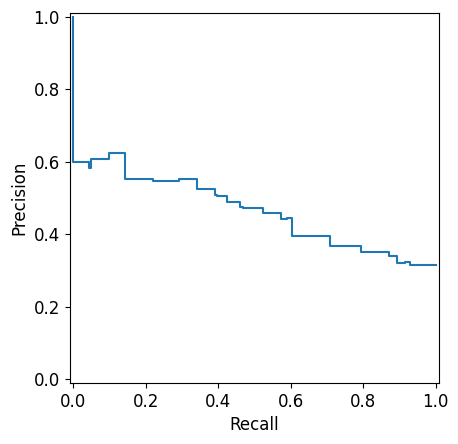
\includegraphics[width=0.45\textwidth]{/files/src/.media/simpleTreeAuprc.png}
    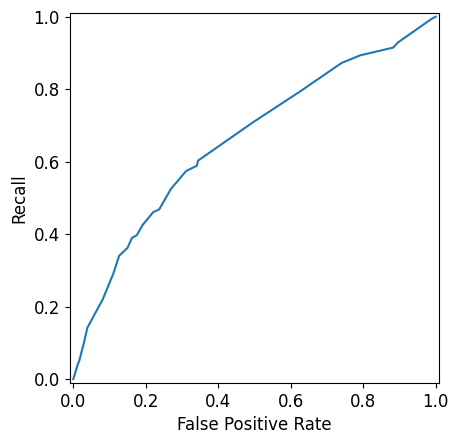
\includegraphics[width=0.45\textwidth]{/files/src/.media/simpleTreeAucroc.png}
    \caption{Curvas \textit{precision-recall}, izquierda, y \textit{receiving operator characteristic}, derecha, para el árbol de decisión \textit{simple}.}
    \label{curvas_simple}
\end{figure}

Es interesante notar que \textit{accuracy} obtuvo un valor más alto que \textit{auprc} y \textit{aucroc} en validación. Esto puede dar cuenta de la incapacidad de \textit{accuracy} para capturar el efecto de los distintos tipos de errores en un problema con clases desbalanceadas. También, parece interesante que \textit{accuracy} obtuvo en validación resultados más variados que las otras métricas. 

Un detalle importante en la interpretación de estos resultados, creemos, es la importancia sobre la decisión de \textit{cuál es la clase positiva}. En particular, \textit{auprc} está sesgado hacia el comportamiento de la clase positiva, mientras que \textit{aucroc} es más imparcial \cite{Saito}. Por otro lado, \textit{auprc} se considera mejor para problemas desbalanceados que \textit{aucroc} \cite{Saito}. Sin embargo, dado que es de interés para el problema el ---\textit{mal pronóstico}---, consideramos que \textit{aucroc} es la medida más adecuada de las tres.

\subsection{Búsqueda en cuadrícula}

Dados los resultados obtenidos, parece interesante explorar otros hiperparámetros para estimar qué tan capaces pueden llegar a ser los \textit{árboles de decisión} para el problema bajo estudio. Para ello, realizaremos una primer búsqueda en cuadrícula con algunos hiperparámetros provistos por la cátedra. En la próxima sección lo complementaremos con una búsqueda aleatoria más extensiva.

En este caso, evaluaremos cada set de hiperparámetros $hs$ en la Figura \ref{grid_search}, aplicando $5$-fold cross-validation estratificado con métrica \textit{accuracy} promedio\footnote{Por decisión de la cátedra para este ejercicio.}.

\vspace{0.5em}
\begin{figure}[!htbp]
    \begin{center}
        \begin{tabular}{ |c|c|c|c| } 
         \hline
        Altura Máxima   & Criterio de corte & Accuracy (train)  & Accuracy (validación) \\
        \hline
        $3$             & Gini              &  $0.8207$         & $0.6905$  \\ 
        $5$             & Gini              &  $0.9126$         & $0.7127$  \\
        $\infty$        & Gini              &  $1.0000$         & $0.6637$  \\ 
        $3$             & Entropía          &  $0.7890$         & $0.6815$  \\
        $5$             & Entropía          &  $0.8937$         & $0.6503$  \\ 
        $\infty$        & Entropía          &  $1.0000$         & $0.6459$  \\ 
        \hline
        \end{tabular}
    \end{center}
    \caption{\textit{Accuracy} promedio resultante de realizar $5$-fold cross-validation estratificado, para \textit{árboles de decisión} con distintos hiperparámetros.} \label{grid_search}
\end{figure}

La figura \ref{grid_search} muestra los resultados obtenidos. Podemos ver una clara tendencia a sobreajustar a medida que aumenta la altura máxima permitida. Por su parte, el criterio Gini obtuvo mejores resultados que Entropía en todas las instancias de evaluación. Algo que llama la atención es que un aumento modesto en la altura máxima permitida (de $3$ a $5$ niveles) causó una mejora en evaluación al usar el criterio Gini, pero un pérdida en el caso de Entropía.
